\begin{center}
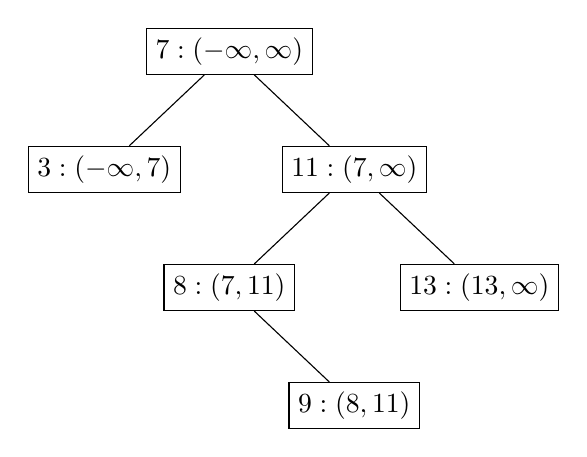
\begin{tikzpicture}[
sibling distance=1.25in,
every node/.style={draw}
]
\node {\(7: (-\infty, \infty)\)}
    child { node {\(3: (-\infty, 7)\)} }
    child { node {\(11: (7, \infty)\)} 
        child { node {\(8: (7, 11)\)}
            child [missing]
            child { node {\(9: (8, 11)\)}}
        }
        child { node {\(13: (13, \infty)\)}}
    };
\end{tikzpicture}
\captionof{figure}{Particionar niveles en intervalos}
\end{center}